\documentclass[../main.tex]{subfiles}

\begin{document}
	\rhead{Hola}
\begin{enumerate}[(a)]

\item Identifique las variables aleatorias y la variable de desempeño utilizadas
para evaluar la decisión.

La única variable de desempeño para la evaluación de una decisión por medio del modelos es la ganancia mensual de la fábrica (pesos).

Las variables aleatorias son:

\begin{itemize}
\item Demanda diaria del plástico impermeable negro de la máquina TX1 $Uniforme(4000, 5000)$.
\item Demanda diaria del plástico impermeable negro de la máquina TX2 $Tri(1200, 1800, 2100)$.
\item Demanda diaria del plástico impermeable amarillo $\mathcal{N} (\mu = 2000 , \sigma = 100)$.
\item Costo de producción del plástico impermeable negro  $\mathcal{N} (\mu = 750 , \sigma = 90)$.
\item Costo de producción del plástico impermeable amarillo.\\
$Uniforme(1100, 1350)$.
\end{itemize}

\item Presente un esquema del modelo determinístico construido para
representar la situación descrita. Utilice los valores esperados de las variables
aleatorias para establecer el valor de la variable de desempeño.

En ambos casos, el valor de venta corresponde al valor de mensual de la venta, igualmente el costo de producción mensual (multiplicando cada valor por 30). El arriendo, se obtiene de la tabla. El costo mensual es la suma de los costos de producción, arriendo y servicios. Por último, la ganancia es el valor por ventas menos los costos operacionales mensuales.

\begin{figure}[h]
\centering
\includegraphics[width=6cm]{fig1-1}
\label{fig:img1}
\caption{Modelo determinístico para la maquina TX-1}
\end{figure}

\begin{figure}[h]
\centering
\includegraphics[width=6cm]{fig1-2}
\label{fig:img1}
\caption{Modelo determinístico para la maquina TX-2}
\end{figure}

Siguiendo el mismo modelo determinístico, se diseñó el probabilista.

\item ¿Cuál es el valor esperado y el coeficiente de variabilidad de la variable
de desempeño en cada alternativa?

A continuación se muestran los resultados de la simulación.

\begin{figure}[h]
\centering
\includegraphics[width=8cm]{fig1-3}
\label{fig:img1}
\end{figure}
\begin{figure}[h]
\centering
\includegraphics[width=4cm]{fig1-5}
\label{fig:img1}
\end{figure}

$$\mathbb{E}(TX_{1}) = 85562109.72 \Rightarrow Coef = \frac{12793316.12}{85562109.72}$$

\pagebreak

\begin{figure}[h]
\centering
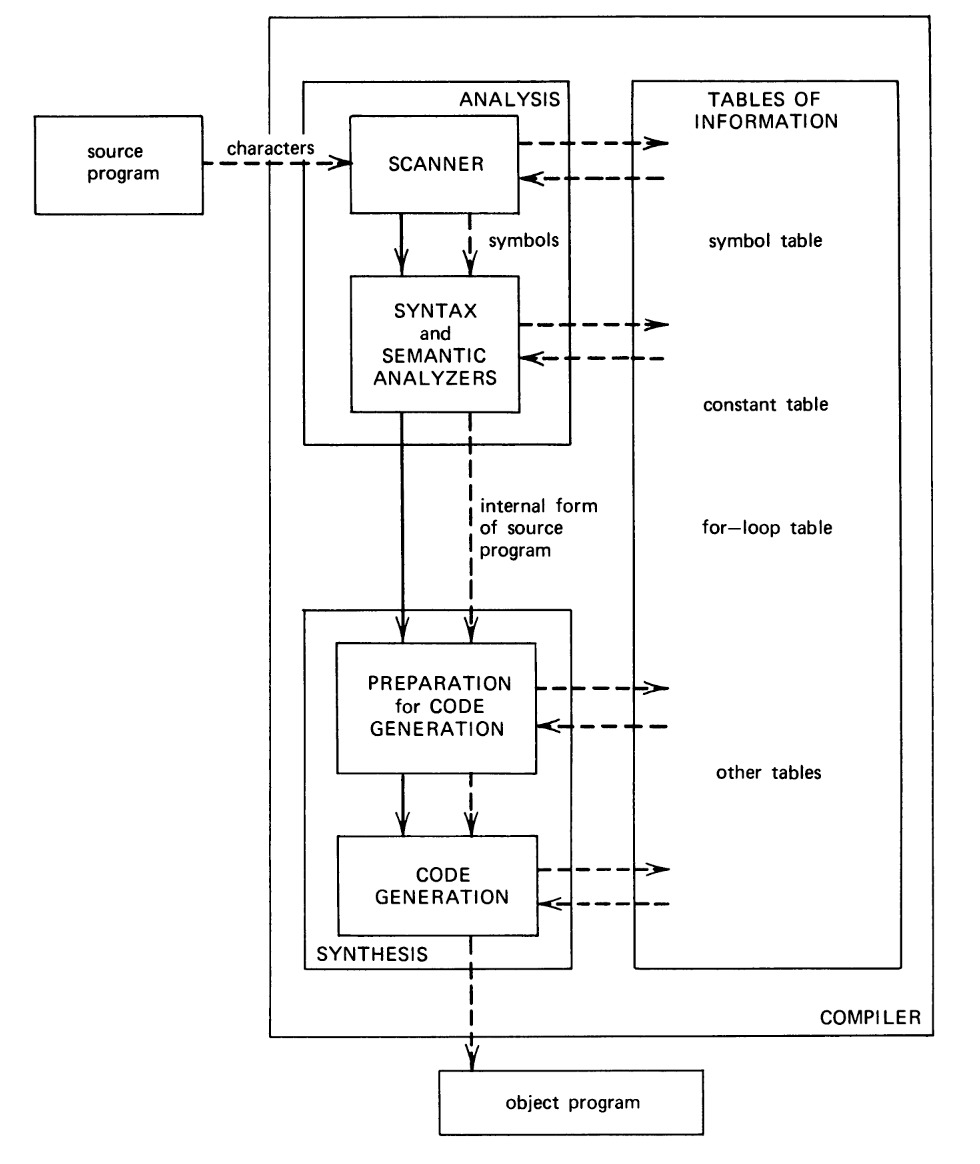
\includegraphics[width=8cm]{fig1-4}
\label{fig:img1}
\end{figure}
\begin{figure}[h]
\centering
\includegraphics[width=4cm]{fig1-6}
\label{fig:img1}
\end{figure}

$$\mathbb{E}(TX_{2}) = 95207785.72 \Rightarrow Coef = \frac{8235361.50}{95207785.72}$$

\pagebreak

\item Calcule un intervalo de confianza con un nivel de confiabilidad del 90\%,
para la variable de desempeño en cada alternativa.

Se muestra el intervalo de confianza en ambas alternativas.

\begin{figure}[h]
\centering
\includegraphics[width=8cm]{fig1-7}
\label{fig:img1}
\end{figure}
\begin{figure}[h]
\centering
\includegraphics[width=8cm]{fig1-8}
\label{fig:img1}
\end{figure}

\pagebreak

\item Encuentre el percentil del 50\% y 90\% para la variable de desempeño de
cada alternativa. Realice una interpretación de cada uno de los percentiles, en cada
una de las variables de desempeño.

\begin{figure}[h]
\centering
\includegraphics[width=6cm]{fig1-9}
\label{fig:img1}
\end{figure}
\begin{figure}[h]
\centering
\includegraphics[width=6cm]{fig1-10}
\label{fig:img1}
\end{figure}

\item ¿Cuál es la probabilidad de obtener utilidades si la compañía decide
arrendar la máquina TX-1? y ¿Cuál es la probabilidad de obtener utilidades si la
compañía decide arrendar la máquina TX-2?

Dados los percentiles anteriores, la probabilidad de no perder dinero es de 1.

\item Realice un análisis de sensibilidad para determinar la variable que más
incide en la variable de desempeño de cada alternativa.

\begin{figure}[h]
\centering
\includegraphics[width=4cm]{fig1-11}
\label{fig:img1}
\end{figure}

\begin{figure}[h]
\centering
\includegraphics[width=4cm]{fig1-12}
\label{fig:img1}
\end{figure}

\pagebreak

\item Realice un gráfico de superposición de los resultados de las alternativas
evaluadas y de acuerdo con este resultado y el de los puntos anteriores, determine
¿cuál es para usted la mejor alternativa? Justifique claramente su respuesta.

\begin{figure}[h]
\centering
\includegraphics[width=8cm]{fig1-13}
\label{fig:img1}
\end{figure}

Aunque la distribución generada para la alternativa de la máquina 1 es menos variable que la otra, es más probable ganar más dinero (la media) con la alternativa de la máquina 2. Por esto, y por nuestra alta aversión al riesgo, se considera elegir la máquina TX-2.

\end{enumerate}
\end{document}
